% Author: Monika Záhradníková <xzahra33>

\documentclass[a4paper, 11pt]{article}
\setlength{\parindent}{2em}

\usepackage[slovak]{babel}
\usepackage[utf8]{inputenc}
\usepackage[left=2cm, top=3cm, text={17cm, 24cm}]{geometry}
\usepackage{times}
\usepackage{array}
\usepackage{verbatim}
\usepackage{enumitem}
\usepackage{xcolor}
\usepackage{soul}
\usepackage{graphicx}
\usepackage[unicode]{hyperref}

\newcommand{\coloredtext}[1]{\textcolor{green!70!black}{#1}}
\newcommand{\highlight}[1]{\colorbox{red!20}{\textcolor{black}{#1}}}

\begin{document}

%%%%%%% Titulná strana %%%%%%%%
    \begin{titlepage}
        \begin{center}
            
\includegraphics[width=0.77\linewidth]{fitlogo.png} \\
    
            \vspace{\stretch{0.382}}
    
            \Huge{Projektová dokumentácia} \\
            \LARGE{\textbf{Implementácia prekladača imperatívneho jazyka IFJ23}} \\
            \Large{Tím xjerab28, varianta vv-BVS}
            \vspace{\stretch{0.618}}
        \end{center}
    
        \begin{minipage}{0.4 \textwidth}
            {\Large \today}
        \end{minipage}
        \hfill
        \begin{minipage}[r]{0.6 \textwidth}
            \Large
            \begin{tabular}{l l l}
                \textbf{Jakub Jeřábek} & \textbf{(xjerab28)} & \quad 25\,\% \\
                Vojtěch Teichmann & (xteich02) & \quad 25\,\% \\
                Doubravka Šimůnková & (xsimun05) & \quad 25\,\% \\
                Monika Záhradníková & (xzahra33) & \quad 25\,\% \\
            \end{tabular}
        \end{minipage}
    \end{titlepage}
    

%%%%%%%% Obsah %%%%%%%%

\pagenumbering{roman}
\setcounter{page}{1}
\tableofcontents
\clearpage


%%%%%%%% Úvod %%%%%%%%%

\pagenumbering{arabic}
\setcounter{page}{1}

\section{Úvod}

Cieľom projektu bolo implementovať prekladač imperatívneho jazyka IFJ23 do~predmetov IFJ~a~IAL.
Zadaným jazykom na~implementáciu bol jazyk~C. Program funguje ako~konzolová aplikácia, ktorá načíta
zdrojový kód napísaný v~jazyku~IFJ23 a~preloží ho do~cieľového jazyka IFJcode23 (medzikód). V~prípade
chyby vracia program odpovedajúcu návratovú hodnotu.


%%%%%%%%%% Návrh a implementácia %%%%%%%%%%%%%

\section{Návrh a~implementácia}

Projekt je zostavený zo~štyroch základných častí, ktoré budú vysvetlené v~nasledujúcich
podkapitolách.

\subsection{Lexikálna analýza}
Začali sme implementáciou lexikálneho analyzátora, ktorý sa nachádza v~súbore~\texttt{scanner.c}.
Lexikálny analyzátor číta zo~štandardného vstupu, ktorý musí obsahovať program napísaný v~jazyku IFJ23. Základom lexikálnej analýzy je deterministický konečný automat (ďalej DKA), ktorého diagram je na~stranách \pageref{figure:DKA1} a \pageref{figure:DKA2}.

Hlavnou funkciou lexikálneho analyzátora je funkcia \texttt{getToken}, ktorá vyžaduje parametre \texttt{token} a \texttt{swiftFile}. Parameter \texttt{swiftFile} je ukazateľ na~vstupný súbor obsahujúci program napísaný v~jazyku IFJ23 a~\texttt{token} je ukazateľ na datovú štruktúru \texttt{Token}.

Funkcia číta každý znak a~cez príkaz \texttt{switch} prechádza do~nasledujúcich stavov (to je definované pomocou DKA). Keď príkaz \texttt{switch} prejde do~stavu, ktorý odpovedá aktuálnemu tokenu (nájde lexikálne správny token), uloží do~parametra \texttt{token} typ tokenu (typy sú definované výčtovým typom \texttt{TokenType}) a~hodnotu tokenu. Analyzátor rozlišuje, či je hodnota tokenu datového typu \texttt{string}, \texttt{int}, \texttt{double}, či je to kľúčové slovo alebo identifikátor. Na~základe toho volá funkciu s prefixom \texttt{process}, ktorá token ďalej spracuje.

Spracovanie escape sekvencií vykonáva funkcia \texttt{processString}, ktorej základom je taktiež konečný automat.

Po dokončení činnosti hlavnej funkcie \texttt{getToken} sa volá funkcia \texttt{handleError}, ktorá vráti odpovedajúci návratový kód a uvoľní alokované prostriedky alebo ,v prípade chyby, program ukončí.

\subsection{Syntaktická a sémantická analýza}
\label{subsec:parser}

Ďalej sme pokračovali implementáciou syntaktického a sémantického analyzátora, ktoré sa nachádzajú
v~súbore \texttt{parser.c}. Syntaktická analýza je založená na~LL -- gramatike (nájdete na~strane \pageref{tab:LL_gram}) a~riadi sa
metódou rekurzívneho zostupu. Týmto postupom sa riadi celá syntaktická analýza okrem spracovania výrazov (bližšie v~podkapitole \ref{subsec:sprac_v} ). Syntaktický a~sémantický analyzátor pracujú zároveň.

Syntaktický analyzátor získava tokeny prostredníctvom lexikálnej analýzy volaním funkcie \texttt{getToken}. Na~základe typu tokena \texttt{tokenType} sa syntaktický analyzátor rozhoduje, ktoré pravidlo LL -- gramatiky použije.

Sémantický analyzátor vykonáva typové kontroly a~pracuje s~tabuľkou symbolov (bližšie popísaná v~podkapitole \ref{subsec:symtable}). Volá operáciu \texttt{symtableInsert}, ktorá ukladá do~tabuľky symbolov identifikátory spolu s~ich vlastnosťami. Zároveň pracuje aj so~zásobníkom tabuliek symbolov \texttt{symStack} (bližšie popísané v~podkapitole \ref{subsec:symstack}).
Pre každý rámec vytvorí jednu tabuľku symbolov a~uloží ju na vrchol zásobníka. Pokiaľ chce nájsť
daný identifikátor v~zásobníku, volá operáciu \texttt{symstackSearchiId}, ktorá prechádza všetky rámce postupne od~vrcholu zásobníka až ku~dnu zásobníka.

Hlavná funkcia celého prekladača \texttt{main} sa nachádza v~súbore \texttt{parser.c}. Tá najprv volá funkciu\\
\texttt{initParser}, ktorá inicializuje parser, tabuľku symbolov pre globálny rámec a~zásobník tabuliek symbolov. Potom funkcia \texttt{initParser} uloží do~tabuľky symbolov všetky vstavané funkcie jazyka IFJ23 za~pomoci funkcie \texttt{buildInFunctions}. Keď funkcia \texttt{initParser} skončí, funkcia \texttt{main} zavolá funkciu \texttt{program}.

\texttt{Program} je najdôležitejšou funkciou v~súbore \texttt{parser.c}. Vyžaduje ako parameter vstupný súbor napísaný v~jazyku IFJ23. Funkcia \texttt{program} na~začiatku vykoná prvý priechod vstupným súborom volaním funkcie \texttt{firstPassage}. V~prvom priechode sa prechádza vstupný súbor a globálny rámec sa naplní \\ deklaráciami funkcií. Súčasne sa prechádza aj konštrukciami \texttt{while} cyklov, ktorých premenné deklerované vnútri cyklu sa ukladajú do~dynamicky alokovaného pola \texttt{whileDefinitions}.

Po prvom priechode sa tabuľka symbolov pre~globálny rámec uloží na~vrchol zásobníka a~inicializuje sa generátor
(bližšie popísaný v~podkapitole \ref{subsec:gen}). Teraz je parser pripravený na~druhý priechod vstupným súborom.

Spracúva telo vstupného súboru volaním rekurzívnej funkcie \texttt{sequenceOrFunction}. Názov funkcie
vypovedá o~tom, že syntaktický analyzátor rozlišuje, či aktuálne spracúva deklaráciu funkcie alebo
sekvenciu príkazov. Pokiaľ sa jedná o~sekvenciu príkazov, volá sa rekurzívna funkcia \texttt{sequence}, v~ktorej
sa syntaktický analyzátor podľa typu tokenu rozhoduje, ktorú funkciu zavolá. Zároveň s~ním samozrejme
pracuje aj sémantický analyzátor, ktorý je popísaný vyššie.

V prípade, že syntaktický analyzátor narazí na~miesto, kde očakáva výraz, predá riadenie precedenčnému syntaktickému analyzátoru implementovanému v~súbore \texttt{expression.c} (bližšie v~podkapitole \ref{subsec:sprac_v}).

Ak syntaktický analyzátor dostáva token, ktorý nevie spracovať na základe pravidiel LL -- gramatiky, ukončuje program vstavanou funkciou v jazyku C \texttt{exit} s~príslušným návratovým kódom.

Pokiaľ sémantický analyzátor narazí na chybu, taktiež ukončuje program funkciou \texttt{exit} s~príslušným návratovým kódom.

\subsubsection{Spracovanie výrazov pomocou precedenčnej syntaktickej analýzy}
\label{subsec:sprac_v}
Ako sme vyššie spomenuli, výrazy spracuje precedenčný syntaktický analyzátor, ktorý je napísaný v~súbore \texttt{expression.c}. Súčasne s~ním vykonáva typové kontroly sémantický analyzátor. Na~začiatku súboru je implementovaná precedenčná tabuľka, ktorú máte možnosť vidieť na strane \pageref{figure:preced_tab}.

Výrazy sa spracujú metódou konvertovania infixu na postfix za~pomoci zásobníka implementovaného v~súbore \texttt{stack.c} (bližšie popísané v~podkapitole \ref{subsec:stack}). Hlavnou funkciou je funkcia \texttt{createExpression}, ktorá
je volaná parserom a~vracia mu datovú štruktúru \texttt{expressionStruct} so~spracovaným výrazom.

Pokiaľ sémantický analyzátor narazí na~nezhodnosť datových typov, ukončuje program vstavanou funkciou \texttt{exit} s~príslušným návratovým kódom.

\subsection{Generátor kódu IFJcode23}
\label{subsec:gen}
Generovanie výstupného kódu IFJcode23 je poslednou časťou našeho prekladača. Generovanie je implementované v súbore \texttt{codeGenerator.c}. Celé generovanie kódu ovláda parser a volá funkcie implementované v \texttt{codeGenerator.c}, aby sa vygeneroval výsledný kód pre určitú sekvenciu príkazov, ktorú aktuálne parser spracoval. 

Ako príklad môžeme uviesť situáciu, kedy parser aktuálne spracúva definíciu funkcie. Po spracovaní hlavičky funkcie zavolá parser funkciu \texttt{generateFunctionHead} a ďalej spracúva telo funkcie. Po spracovaní tela volá parser funkciu \texttt{generateFunctionEnd}. V tomto čase by mala byť vygenerovaná celá funkcia. Obdobne parser volá generátor pri všetkých príkazoch jazyka IFJ23.

V našom projekte sme nepoužili trojadresný kód, ale prevod na postfixový tvar. Pokiaľ parser aktuálne spracúva výraz a príde čas na generovanie kódu, zavolá funkciu \texttt{generateExpression} s parametrom \texttt{expression}, čo je štruktúra obsahujúca postfixový výraz a informácie o premenných.

Pri generovaní premenných, či návestí podmienok a cyklov je ako ďalší parameter predávaný\\ \texttt{labelIndex}, ktorý slúži k univerzálnej identifikácií premenných, i keď je premenná deklarovaná v globálnom a zároveň v lokálnom rámci. To umožňuje efektívnu prácu so všetkými premennými, ktoré se môžu nachádzať v rôznych rámcoch.

V súbore \texttt{codeGenerator.c} sú implementované aj dve dôležité funkcie \texttt{comment} a \texttt{inst}, ktoré generátor využíva na výpis komentárov a jednotlivých inštrukcií.


%%%%%%%%%% Použité algoritmy a datové štruktúry %%%%%%%%%%%%%

\section{Použité algoritmy a~datové štruktúry}

\subsection{Tabuľka symbolov}
\label{subsec:symtable}
    Tabuľku symbolov sme implementovali v~súbore \texttt{symtable.c} podľa varianty zadania, ktoré sme si vybrali. Zvolili sme výškovo-vyvážený binárny vyhľadávací strom (ďalej BST). Pri~implementácií BST sme postupovali podľa prednášaných techník z~predmetu~IAL.
    
    Vytvorili sme si datovú štruktúru \texttt{Tnode}, ktorá popisovala uzol BST. V~každom uzle sme ukladali názov identifikátora ako kľúč \texttt{key}. Všetky vlastnosti identifikátora, ktoré sémantická analýza potrebovala
    pre~prácu s~identifikátorom, sme ukladali do~datovej štruktúry \texttt{Tdata}.


\subsection{Zásobník symbolov pre~precedenčnú syntaktickú analýzu}
\label{subsec:stack}
    Na~to, aby mohla precedenčná syntaktická analýza konvertovať výraz zadaný v~infixovom tvare na~tvar postfixový, sme potrebovali implementovať zásobník. Tu sa symboly ukladajú na~vrchol zásobníka a~naopak odstraňujú z~vrcholu zásobníka na~základe pravidiel precedenčnej tabuľky (na strane \pageref{figure:preced_tab}), ktorá hovorí o~tom,
    ktorý symbol má vyššiu prioritu.
    
    Zásobník je implementovaný v~súbore \texttt{stack.c} a pri~implementácií sme sa nechali inšpirovať metódami
    prebranými na~prednáškach predmetu IAL.
    

\subsection{Zásobník tabuliek symbolov}
\label{subsec:symstack}
    Ďalší zásobník, ktorý sme museli implementovať, bol zásobník tabuliek symbolov, ktorý sa nachádza v~súbore \texttt{symstack.c}. Potrebovali sme ho, aby sémantický analyzátor dokázal rozlišovať, ktoré identifikátory
    (premenné) sa nachádzajú v~ktorom rámci. Každý prvok zásobníka je vlastne odkaz na~tabuľku symbolov pre globálny alebo lokálny rámec.
    
    So zásobníkom sa dajú vykonávať klasické operácie preberané aj na~prednáškach z IAL. Výnimkou je
    funkcia \texttt{symstackSearchiId}, ktorá bola už popísaná vyššie v~podkapitole \ref{subsec:parser}.

\subsection{Dynamický reťazec}

    Dynamický reťazec a~operácie nad~ním sme implementovali v~súbore \texttt{string.c}. Vytvorili sme štruktúru \texttt{String}, do~ktorej sa postupne ukladá reťazec tokenov, o~ktorom lexikálna analýza dopredu nevie, koľko bude mať znakov. Ďalej sa do~štruktúry ukladá veľkosť už~alokovanej pamäte pre~reťazec a~aktuálna dĺžka reťazca.

    Z operácií nad~dynamickým stringom môžeme spomenúť operáciu \texttt{addCharStr}, ktorá pridá na~koniec dynamického reťazca nový znak alebo operáciu \texttt{addStrStr}, ktorá pridá na~koniec dynamického reťazca nový reťazec.

    Operácie nad dynamickým stringom volá lexikálna analýza a generátor kódu.

%%%%%%%%%% Práca v tíme %%%%%%%%%%%%%

\section{Práca v~tíme}
\subsection{Spôsob práce v~tíme a~komunikácia}
Na~začiatku projektu sme sa osobne stretli a prediskutovali, akým spôsobom budeme pracovať.
Stanovili sme si, že chceme mať projekt hotový už pred pokusným odovzdávaním. Dohodli sme sa na~stretávaní minimálne raz týždenne, kde sme si vždy zhrnuli, ako sme pokročili v práci, poprípade sme
programovali a snažili sa nájsť riešenie problémov. Pokiaľ nebolo možné osobné stretnutie, stretli sme sa
online cez~hovor, prostredníctvom Discordu.

Pre~prehľadnosť informácií ohľadom projektu (hlavne v~začiatkoch) sme využívali software Padlet,
kde sme si vytvorili zdieľanú nástenku a~ukladali sem všetky potrebné informácie.

\subsection{Verzovací systém}
Pre~správu verzií sme využili verzovací systém Git, s~ktorým sme už mali skúsenosti. GitHub nám umožnil vytvoriť zdieľaný repozitár, a~tak sme mohli pracovať na~viacerých úlohách súčasne. Zo~začiatku sme pracovali na~hlavnej vetve, neskoršie sme prešli k~práci na~vedľajších vetvách, ktoré nám poskytovali istotu, že prípadné problémy nebudú zavedené do~už fungujúceho programu.

\subsection{Rozdelenie práce medzi členov}
Rozdelenie práce neprebehlo hneď na~začiatku, ale vyvíjalo sa postupne pri~práci na~projekte.
Práca bola rozdelená následovne:

\subsection*{\underline{Jakub Jeřábek:}}
\begin{itemize}
  \item Vedenie tímu
  \item Implementácia lexikálneho analyzátora
  \item Implementácia parseru
  \item Implementácia generátora kódu
  \item Testovanie
\end{itemize}

\subsection*{Doubravka Šimůnková:}
\begin{itemize}
  \item Návrh LL -- gramatiky 
  \item Návrh LL -- tabuľky
  \item Návrh precedenčnej tabuľky
  \item Implementácia parseru
  \item Testovanie
\end{itemize}

\subsection*{Vojtěch Teichmann:}
\begin{itemize}
  \item Návrh automatu pre lexikálnu analýzu
  \item Implementácia spracovania výrazov
  \item Testovanie
\end{itemize}

\subsection*{Monika Záhradníková:}
\begin{itemize}
  \item Organizácia stretnutí
  \item Implementácia tabuľky symbolov
  \item Implementácia zásobníka symbolov
  \item Testovanie
  \item Dokumentácia, prezentácia
\end{itemize}


\subsection{Problémy}
Ako v~každom tímovom projekte, aj u~nás sa vyskytlo zopár problémov, ktoré sme nevedeli hneď vyriešiť. 

Problém nám robili deklarácie premenných vo~\texttt{while} cykloch, čo sme vyriešili spracovaním týchto deklarácií už v~prvom priechode programom.

Ďalším problémom bolo napojenie tabuľky symbolov a~zásobníka tabuliek symbolov na~parser. Program nám veľa krát hlásil chybu \texttt{segmentation fault} tj. neoprávnený prístup do~pamäte. Nakoniec sme to vyriešili spoločne na~stretnutí.

Problém nám robil taktiež fakt, že znak \texttt{EOL} sa môže nachádzať na akomkoľvek mieste vo~vstupnom súbore. Riešením bolo pridanie tokenu \texttt{EOL} do~výčtového typu \texttt{TokenType} a~zmena LL -- gramatiky.

Nakoniec by sme ako problém spomenuli prípady, kedy parser nedokázal jednoznačne určiť len na~základe aktuálneho tokenu, ktoré pravidlo má použiť. V niektorých prípadoch sa napríklad parser potreboval pozrieť do~tabuľky symbolov, aby mohol vybrať pravidlo LL -- gramatiky na~základe toho, či je aktuálny identifikátor identifikátorom premennej alebo funkcie. Kvôli tomuto problému sme do~LL -- gramatiky zaviedli nedeterministické pravidlá, ktoré sú v~LL -- gramatike (na strane \pageref{tab:LL_gram}) vyznačené na~červeno.

%%%%%%%%%% Záver %%%%%%%%%%%%%

\section{Záver}
Zo~začiatku bolo veľmi náročné preniesť všetky informácie z~prednášaných látok do~projektu a~predstaviť si, ako to má celé fungovať. Postupom času sme prišli na~spôsob, ako implementovať jednotlivé časti tak, aby spolu dokázali komunikovať a~vytvoriť tak celok, ktorým je prekladač. Určite nás to veľa naučilo a dalo nám kopec skúseností či už v samotnom programovaní, v~problematike prekladačov alebo v~tímovej práci.

\subsection{Zdroje}
Ako zdroje sme využívali výukové materiály predmetov IFJ a~IAL. Informácie sme čerpali hlavne z~demo cvičení, prednášok a~prezentácií.

%%%%%%%%%% Prílohy %%%%%%%%%%%%%
\clearpage

\section{Prílohy}
    \begin{figure}[!ht]
        \centering
        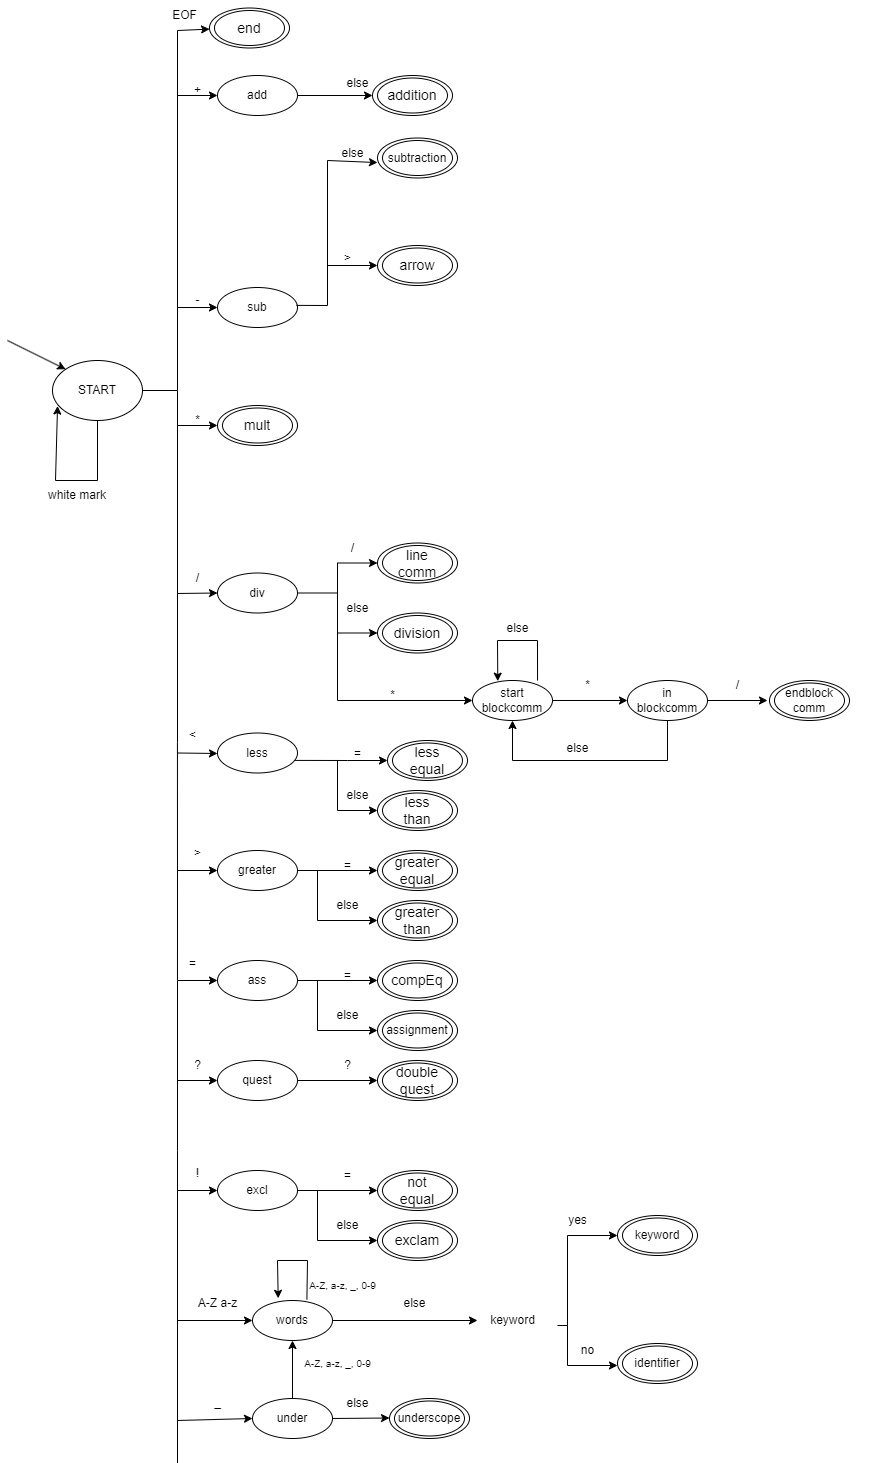
\includegraphics[width=0.75\linewidth]{ka1.png}
        \caption{Diagram konečného automatu špecifikujúci lexikálnu analýzu (1. časť)}
        \label{figure:DKA1}
    \end{figure}

    \begin{figure}[!ht]
        %\centering
        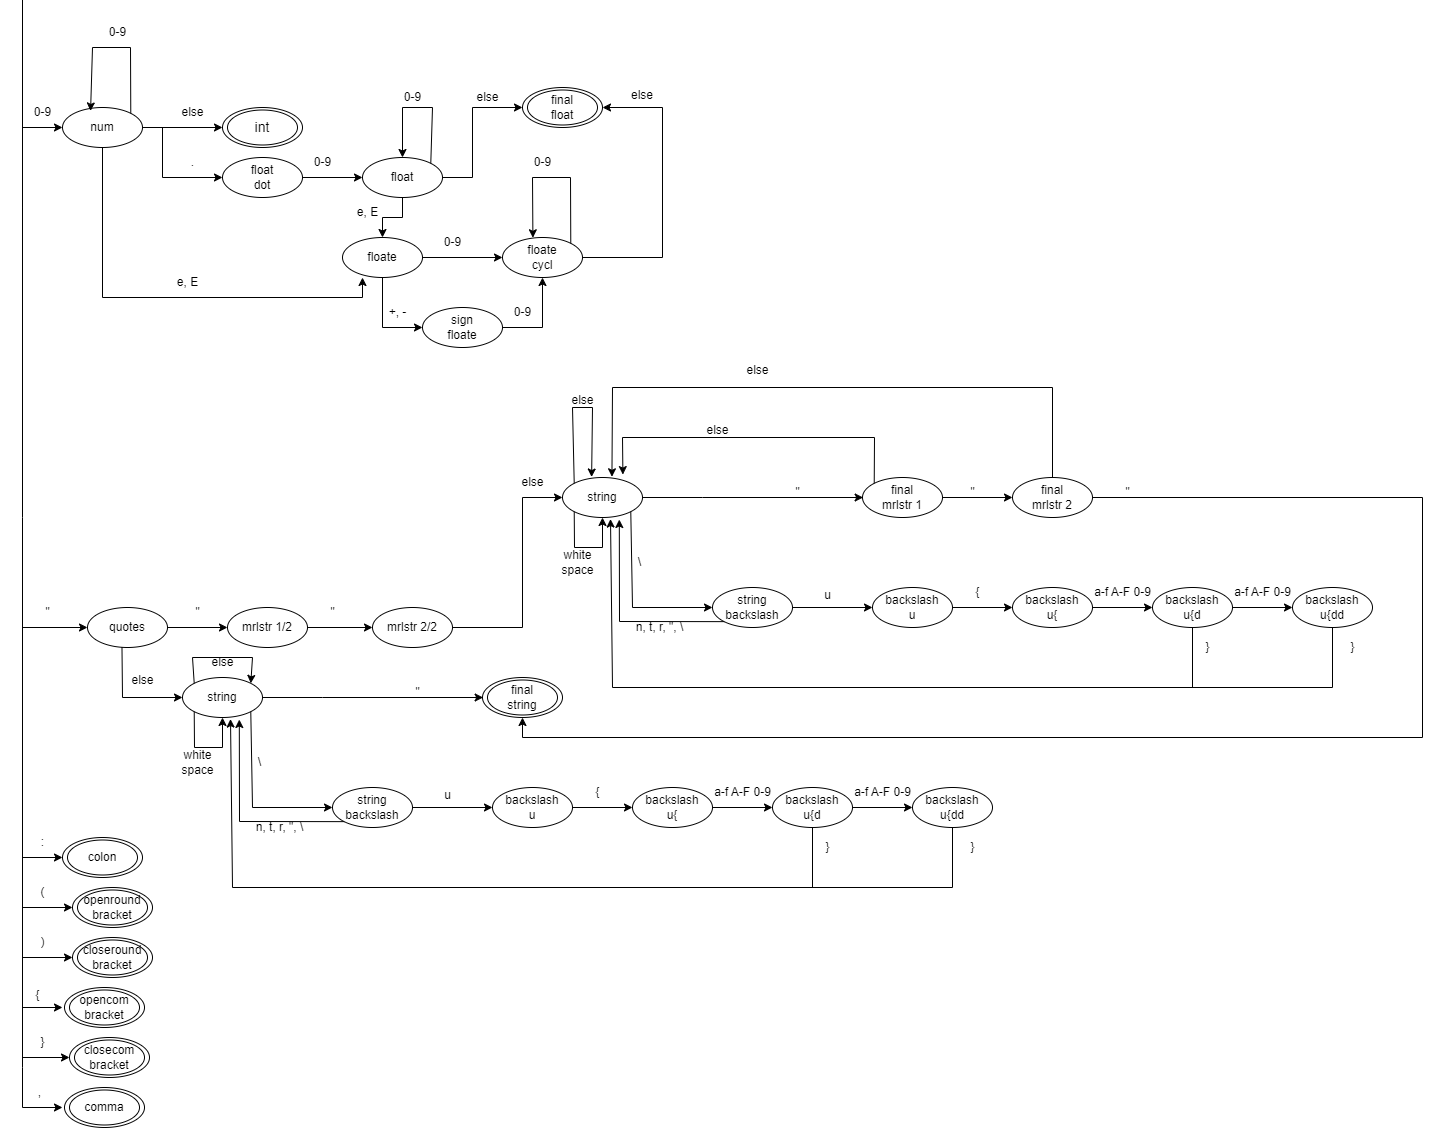
\includegraphics[width=1\linewidth, height=1\linewidth]{ka2.png}
        \caption{Diagram konečného automatu špecifikujúci lexikálnu analýzu (2. časť)}
        \label{figure:DKA2}
    \end{figure}

    \begin{figure}[!ht]
        %\centering
        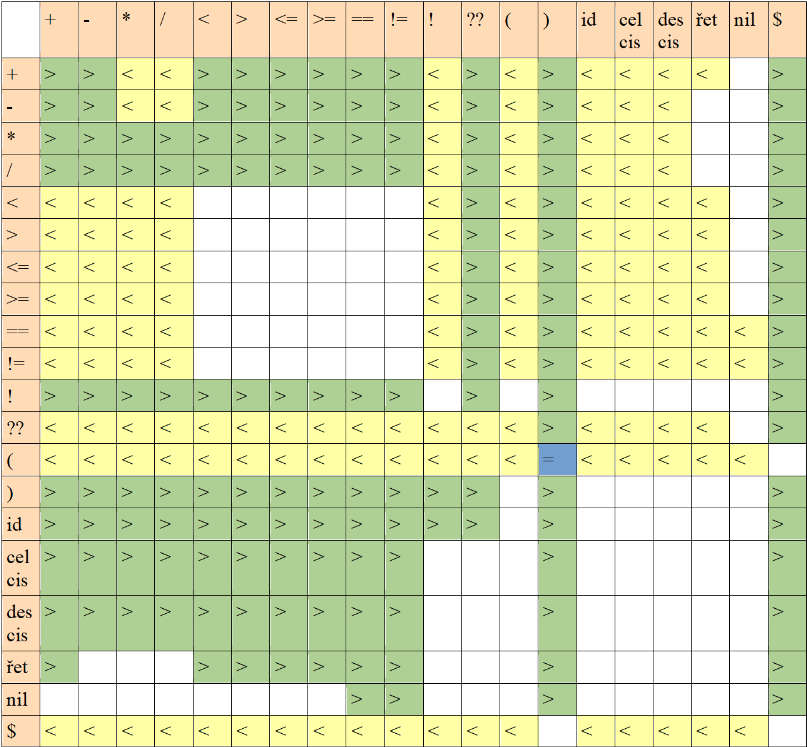
\includegraphics[width=1\linewidth, height=1\linewidth]{precedencni_tab.png}
        \caption{Precedenčna tabuľka špecifikujúca precedenčnú syntaktickú analýzu pre spracovanie výrazov}
        \label{figure:preced_tab}
    \end{figure}
    
\clearpage
    \begin{table}[!ht]
      \centering
      \begin{tabular}{|c|p{4,5cm}|p{11cm}|}
        \hline
        1. & \texttt{[program]} & \texttt{[enter] [sequenceOrFunction]  \coloredtext{EOF}} \\
        \hline
        2. & \texttt{[sequenceOrFunction]} & \texttt{\coloredtext{epsilon}} \\
        \hline
        3. & \texttt{[sequenceOrFunction]} & \texttt{[sequence] [sequenceOrFunction]} \\
        \hline
        4. & \texttt{[sequenceOrFunction]} & \texttt{\coloredtext{Func} [enter] \coloredtext{id} [enter] \coloredtext{(}[enter] [listOfParams]\coloredtext{)} [enter][returnType] \coloredtext{\{}[enter] [sequence]\coloredtext{\}} \coloredtext{EOL} [enter] [sequenceOrFunction]} \\
        \hline
        5. & \texttt{[sequence]} & \texttt{\coloredtext{epsilon}} \\
        \hline
        6. & \texttt{[sequence]} & \texttt{[initType] [enter] \coloredtext{id} [enter] [determineType] \coloredtext{EOL} [enter] [sequence]} \\
        \hline
        7. & \texttt{[sequence]} & \texttt{\coloredtext{If} [enter] [statement] \coloredtext{\{}[enter] [sequence]\coloredtext{\}} [enter] \coloredtext{else} [enter] \coloredtext{\{}[enter] [sequence]\coloredtext{\}} \coloredtext{EOL} [enter] [sequence]} \\
        \hline
        8. & \texttt{[sequence]} & \texttt{\coloredtext{While} [enter] [expression] \coloredtext{\{}[enter] [sequence]\coloredtext{\}} \coloredtext{EOL} [enter] [sequence]} \\
        \hline
        9. & \texttt{\highlight{[sequence]}} & \texttt{\highlight{\coloredtext{Id} [enter] \coloredtext{=} [enter] [valueToVariable] \coloredtext{EOL}} \highlight{[enter] [sequence]}} \\
        \hline
        10. & \texttt{\highlight{[sequence]}} & \texttt{\highlight{[callingFunction] \coloredtext{EOL} [enter] [sequence]}} \\
        \hline
        11. & \texttt{[sequence]} & \texttt{\coloredtext{Return} [returnExpression] \coloredtext{EOL} [enter] [sequence]} \\
        \hline
        12. & \texttt{[initType]} & \texttt{\coloredtext{Var}} \\
        \hline
        13. & \texttt{[initType]} & \texttt{\coloredtext{Let}} \\
        \hline
        14. & \texttt{[returnExpression]} & \texttt{\coloredtext{epsilon}} \\
        \hline
        15. & \texttt{[returnExpression]} & \texttt{[expression]} \\
        \hline
        16. & \texttt{[listOfParams]} & \texttt{\coloredtext{epsilon}} \\
        \hline
        17. & \texttt{[listOfParams]} & \texttt{[parameter][parameters]} \\
        \hline
        18. & \texttt{[parameters]} & \texttt{\coloredtext{,} [parameter][parameters]} \\
        \hline
        19. & \texttt{[parameters]} & \texttt{\coloredtext{epsilon}} \\
        \hline
        20. & \texttt{[[parameter]} & \texttt{[name][name]\coloredtext{:}[type] [enter]} \\
        \hline
        21. & \texttt{[name]} & \texttt{\coloredtext{Id} [enter]} \\
        \hline
        22. & \texttt{[name]} & \texttt{\coloredtext{\_} [enter]} \\
        \hline
        23. & \texttt{[returnType]} & \texttt{\coloredtext{epsilon}} \\
        \hline
        24. & \texttt{[returnType]} & \texttt{\coloredtext{->} [enter] [type]} \\
        \hline
        25. & \texttt{[type]} & \texttt{\coloredtext{Double}} \\
        \hline
        26. & \texttt{[type]} & \texttt{\coloredtext{Double?}} \\
        \hline
        27. & \texttt{[type]} & \texttt{\coloredtext{Int}} \\
        \hline
        28. & \texttt{[type]} & \texttt{\coloredtext{Int?}} \\
        \hline
        29. & \texttt{[type]} & \texttt{\coloredtext{String}} \\
        \hline
        30. & \texttt{[type]} & \texttt{\coloredtext{String?}} \\
        \hline
        31. & \texttt{[determineType]} & \texttt{\coloredtext{=} [enter] [valueToVariable]} \\
        \hline
        32. & \texttt{[determineType]} & \texttt{\coloredtext{:} [enter] [type] [possibleExpression]} \\
        \hline
        33. & \texttt{[possibleExpression]} & \texttt{\coloredtext{=} [enter] [valueToVariable]} \\
        \hline
        34. & \texttt{[possibleExpression]} & \texttt{\coloredtext{epsilon}} \\
        \hline
        35. & \texttt{[statement]} & \texttt{[expression]} \\
        \hline
        36. & \texttt{[statement]} & \texttt{\coloredtext{Let} [enter] \coloredtext{id} [enter]} \\
        \hline
        37. & \texttt{\highlight{[valueToVariable]}} & \texttt{\highlight{[expression]}} \\
        \hline
        38. & \texttt{\highlight{[valueToVariable]}} & \texttt{\highlight{[callingFunction]}} \\
        \hline
        
      \end{tabular}
      \caption{LL -- gramatika riadiaca syntaktickú analýzu (1. časť)}
      \label{tab:LL_gram}
    \end{table}

\clearpage
    \begin{table}[!ht]
      \centering
      \begin{tabular}{|c|p{4,5cm}|p{11cm}|}
        \hline
        39. & \texttt{[callingFunction]} & \texttt{\coloredtext{Id} [enter]\coloredtext{(}[enter][listOfEnterParams]\coloredtext{)}} \\
        \hline
        40. & \texttt{[listOfEnterParams]} & \texttt{\coloredtext{epsilon}} \\
        \hline
        41. & \texttt{[listOfEnterParams]} & \texttt{[enterParameter][enterParameters]} \\
        \hline
        42. & \texttt{[enterParameters]} & \texttt{\coloredtext{,} [enter][enterParameter][enterParameters]} \\
        \hline
        43. & \texttt{[enterParameters]} & \texttt{\coloredtext{epsilon}} \\
        \hline
        44. & \texttt{[enterParameter]} & \texttt{[nameParameter][term]} \\
        \hline
        45. & \texttt{\highlight{[nameParameter]}} & \texttt{\highlight{\coloredtext{Id} [enter]\coloredtext{:} [enter]}} \\
        \hline
        46. & \texttt{\highlight{[nameParameter]}} & \texttt{\highlight{\coloredtext{epsilon}}} \\
        \hline
        47. & \texttt{[term]} & \texttt{\coloredtext{id}} \\
        \hline
        48. & \texttt{[term]} & \texttt{\coloredtext{Deset.cislo}} \\
        \hline
        49. & \texttt{[term]} & \texttt{\coloredtext{Cele.cislo}} \\
        \hline
        50. & \texttt{[term]} & \texttt{\coloredtext{retezec}} \\
        \hline
        51. & \texttt{[term]} & \texttt{\coloredtext{nil}} \\
        \hline
        52. & \texttt{[enter]} & \texttt{\coloredtext{epsilon}} \\
        \hline
        53. & \texttt{[enter]} & \texttt{\coloredtext{EOL}[enter]} \\
        \hline
    \end{tabular}
    \caption{LL -- gramatika riadiaca syntaktickú analýzu (2. časť)}
\end{table}

\clearpage
    \begin{figure}[!ht]
        %\centering
        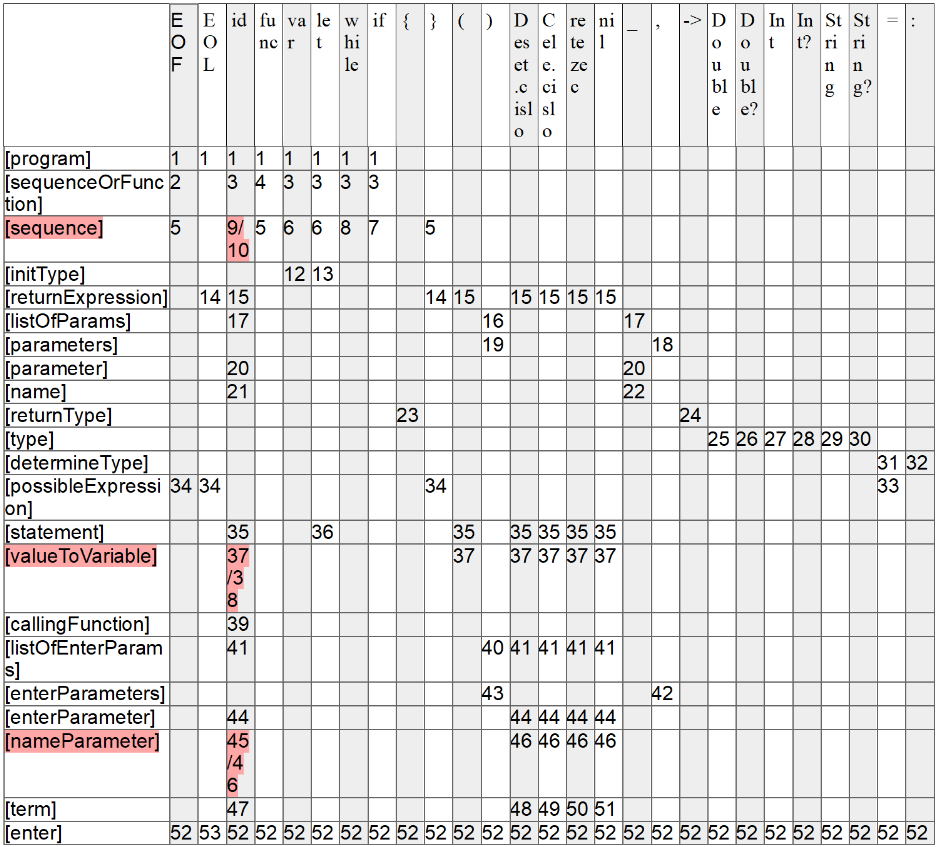
\includegraphics[width=1\linewidth, height=1\linewidth]{lltabulka.png}
        \caption{LL -- tabuľka použitá pri syntaktickej analýze}
        \label{figure:LL_tab}
    \end{figure}



\end{document}